\subsection{Polynomials}

\frame{

\frametitle{\secname: \subsecname}
\begin{columns}
\column{0.5\textwidth}
\begin{figure}
\centering
\begin{tikzpicture}[every node/.style={inner sep=0pt}]
\colorlet{coeff}{alerted text.fg}
\definecolor{term}{HTML}{9900ff}
\definecolor{deg}{HTML}{0000cc}
\node (f) {$f(x)$};
\node (f0)[right=0pt of f.base east,anchor=base west] {$\null=3+2x$};
\node (f1)[right=0pt of f0.base east,anchor=base west] {$\null-4$};
\node (f2)[right=0pt of f1.base east,anchor=base west] {$x^2$};
\node (f3)[right=0pt of f2.base east,anchor=base west] {$\null+x$};
\node (f4)[right=0pt of f3.base east,anchor=base west] {$^3$};
\node (coeffbox) [fit=(f1),draw,inner sep=1pt,color=coeff,thick] {};
\node (termbox) [fit=(f1)(f2),draw,inner sep=3pt,color=term,thick] {};
\node (degbox) [fit=(f4),draw,inner sep=1pt,color=deg,thick] {};
\node (coefflab) [above left=of coeffbox,draw,inner sep=3pt,color=coeff,thick] {coefficient};
\node (termlab) [above=of termbox,draw,inner sep=3pt,color=term,thick] {term};
\node (deglab) [above right=of degbox,draw,inner sep=3pt,color=deg,thick] {degree};
\draw[color=coeff,thick] (coeffbox) -- (coefflab);
\draw[color=term,thick] (termbox) -- (termlab);
\draw[color=deg,thick] (degbox) -- (deglab);
\end{tikzpicture}
\begin{align*}
f(0)&=3\\
f(1)&=2\\
f(2)&=-1\\
f(3)&=0
\end{align*}
Evaluating a polynomial at a point\\ takes $O(n)$ time
\end{figure}

\column{0.5\textwidth}
\begin{figure}
\centering
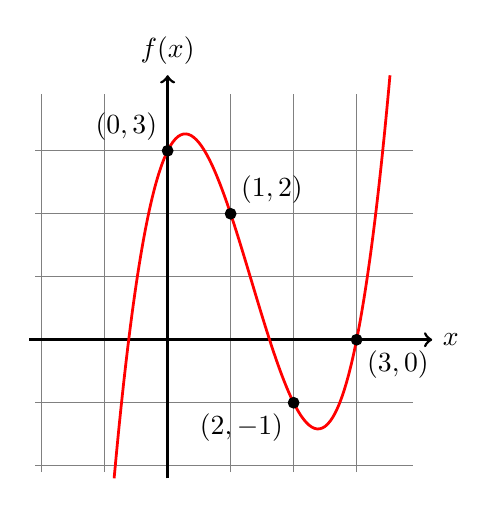
\begin{tikzpicture}[scale=0.8,line width=1pt]
\def\funcpoly{3+2*\x-4*\x*\x+\x*\x*\x}
\draw[very thin,color=gray] (-2.1,-2.1) grid (3.9,3.9);
\draw[->] (-2.2,0) -- (4.2,0) node[right] {$x$};
\draw[->] (0,-2.2) -- (0,4.2) node[above] {$f(x)$};
\draw[color=red,smooth,every node/.style={color=black},mark=*,mark size=2pt,mark options={color=black}]
    plot[domain=-0.84962:0,mark=] (\x,\funcpoly)
    node[above left] {$(0,3)$}
    plot[domain=0:1,mark indices=1] (\x,\funcpoly)
    node[above right] {$(1,2)$}
    plot[domain=1:2,mark indices=1] (\x,\funcpoly)
    node[below left] {$(2,-1)$}
    plot[domain=2:3,mark indices=1] (\x,\funcpoly)
    node[below right] {$(3,0)$}
    plot[domain=3:3.5297,mark indices=1] (\x,\funcpoly)
    ;
\end{tikzpicture}
\end{figure}
\end{columns}

}